\chapter{Preliminaries}
\label{Preliminaries}

\section{Combinatorics}
\subsection{Graphs}

\paragraph{}
The definitions are inspired by~\cite{diestel2017graph}. There are two meanings of the word \textit{graph}. The former  describes a particular type of structure that was originally studied and the latter describes the whole family of various objects that derives from the original definition. Here we study the multigraphs. The original graphs are a special case of multigraphs but the multigraphs are in the big family of graphs.

\begin{definition}[Labeled multigraph]
  \index{graph}
  \index{multigraph}
  \index{labeled graph}
  \index{vertex}
  \index{edge}
  \index{label}
  A \textit{labeled multigraph} is a triple $G = (V, E, L)$ of sets. The set $V$ is the set of \textit{vertices}, $E$ for the \textit{edges} and $L$ for the \textit{labels}. Each edge $e \in E$ is associated with one vertex or a set of two distinct vertices and a label, thus $e \in (V \cup [V]^2) \times L$ where $[V]^2$ is the set of all sets of size two of $V$ i.e. $[V]^2 = \{\#S = 2 | S \in P(V)\}$.
\end{definition}

\paragraph{}
This definition is general and often some simpler definitions of graphs are used. Here are the most common definitions:

\begin{definition}[Unlabeled multigraph]
  \index{unlabeled graph}
  The definition of an \textit{unlabeled multigraph} is similar to the definition a labeled multigraph but without the set of labels $L$. It can be seen as a labeled multigraph with only one label i.e. $\# L = 1$.
\end{definition}

\paragraph{}
We have multiple definitions for different types of multigraphs. The term \textit{multigraph} is used to describe labeled multigraph as well as unlabeled multigraph.

\begin{definition}[Multigraph without loops]
  \index{graph without loops}
  A \textit{multigraph without loops} is a multigraph where the vertices must not be associated with a single vertex. Thus every edge must be associated with a set of two vertices.
\end{definition}

\paragraph{}
Now we give the definition of a graph (here we are talking about the original concept):

\begin{definition}[Graph]
  \index{graph}
  A graph is a multigraph where all the edges must be associated with different vertices or different pair of vertices.
\end{definition}

\begin{definition}[Simple graph]
  \index{simple graph}
  A \textit{simple graph} is an unlabeled graph without loops.
\end{definition}

\paragraph{}
Generally, when the context is clear, the word \textit{graph} is used to talk about any structure in the family and not for this special case.

\paragraph{}
\textbf{Graph drawing}

\paragraph{}
Graphs are often represented as drawings.  Each vertex is represented by a dot. An edge is represented by a line between the two dots that compose it.

\paragraph{}
For example, a graph with $V = \{1,2,3,4\}$ and $E = \{\{1,2\}, \{2,3\}, \{3,4\}, \{1,3\}\}$ can be drawn as:

\begin{figure}[H]
  \begin{center}
    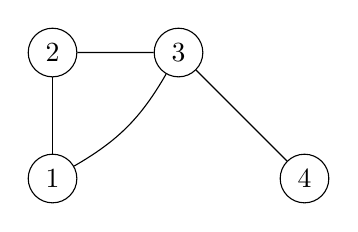
\begin{tikzpicture}[scale=.8]

      \begin{scope}[every node/.style={circle,draw}]
        \node (1)  at (0,0) {1};
        \node (2)  at (0,2) {2};
        \node (3)  at (2,2) {3};
        \node (4)  at (4,0) {4};
      \end{scope}


      \begin{scope}[every edge/.style={draw}]
        \path (1)  edge node {} (2);
        \path (2)  edge node {} (3);
        \path (3)  edge[bend left=15] node {} (1);
        \path (3)  edge node {} (4);
      \end{scope}

    \end{tikzpicture}
    \caption{Example of a representation of a graph}
  \end{center}
\end{figure}

\paragraph{}
The drawing of a graph is obviously not unique.

\paragraph{}
If not needed, the numbers of the vertices on the graphs are often omitted.


\begin{figure}[H]
  \begin{center}
    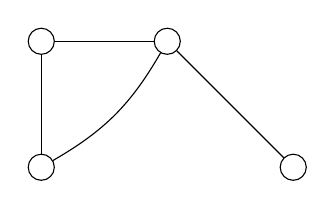
\begin{tikzpicture}[scale=.8]

      \begin{scope}[every node/.style={circle,draw}]
        \node (1)  at (0,0) {};
        \node (2)  at (0,2) {};
        \node (3)  at (2,2) {};
        \node (4)  at (4,0) {};
      \end{scope}


      \begin{scope}[every edge/.style={draw}]
        \path (1)  edge node {} (2);
        \path (2)  edge node {} (3);
        \path (3)  edge[bend left=15] node {} (1);
        \path (3)  edge node {} (4);
      \end{scope}

    \end{tikzpicture}
    \caption{Example of a representation of a graph}
  \end{center}
\end{figure}

\paragraph{}
When a labeled graph is drawn, the labels are written on the edge.

\begin{figure}[H]
  \begin{center}
    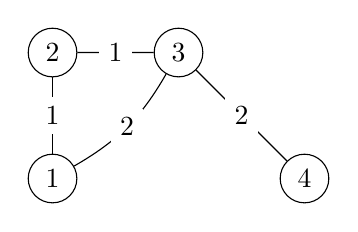
\begin{tikzpicture}[scale=.8]

      \begin{scope}[every node/.style={circle,draw}]
        \node (1)  at (0,0) {1};
        \node (2)  at (0,2) {2};
        \node (3)  at (2,2) {3};
        \node (4)  at (4,0) {4};
      \end{scope}

      \begin{scope}[every node/.style={fill=white}]
        \begin{scope}[every edge/.style={draw}]
          \path (1)  edge node {1} (2);
          \path (2)  edge node {1} (3);
          \path (3)  edge[bend left=15] node {2} (1);
          \path (3)  edge node {2} (4);
        \end{scope}
      \end{scope}

    \end{tikzpicture}
    \caption{Example of a labeled graph}
  \end{center}
\end{figure}

\begin{figure}[H]
  \begin{center}
    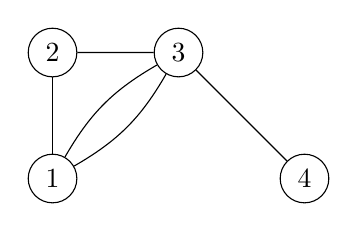
\begin{tikzpicture}[scale=.8]

      \begin{scope}[every node/.style={circle,draw}]
        \node (1)  at (0,0) {1};
        \node (2)  at (0,2) {2};
        \node (3)  at (2,2) {3};
        \node (4)  at (4,0) {4};
      \end{scope}


      \begin{scope}[every edge/.style={draw}]
        \path (1)  edge node {} (2);
        \path (2)  edge node {} (3);
        \path (3)  edge[bend left=15] node {} (1);
        \path (3)  edge[bend right=15] node {} (1);
        \path (3)  edge node {} (4);
      \end{scope}

    \end{tikzpicture}
    \caption{Example of a multigraph}
  \end{center}
\end{figure}
